\documentclass[reprint,amsmath,amssymb,aps,showpacs,superscriptaddress,prl]{revtex4-1}

\usepackage{graphicx}
\usepackage{bm}
\usepackage{epsfig}
\usepackage{amssymb}
\usepackage{amsfonts}
\usepackage{braket}
\usepackage{color}
\usepackage{epstopdf}
\epstopdfsetup{update}
\usepackage{hyperref}
\usepackage{float}
\restylefloat{table}
\usepackage{bibentry}
\usepackage{multirow}
\usepackage[caption=false]{subfig}
\newcommand{\ba}{\begin{eqnarray}}
\newcommand{\ea}{\end{eqnarray}}
\newcommand{\bd}{\begin{displaymath}}
\renewcommand{\v}[1]{{\bf #1}}
\newcommand{\nn}{\nonumber \\}

\graphicspath{{figures/}}% Put all figures in this directory.

\begin{document}
%
\title{Machine Learning Application to Two-Dimensional Dzyaloshinskii-Moriya Ferromagnets}

\author{Vinit Kumar Singh}
\email[Electronic address:$~~$]{vinitsingh911@gmail.com}
\affiliation{Department of Physics, Indian Institute of Technology, Kharagpur 721302, India}
\author{Jung Hoon Han}
\email[Electronic address:$~~$]{hanjemme@gmail.com}
\affiliation{Department of Physics, Sungkyunkwan University, Suwon 16419, Korea}
\date{\today}

\begin{abstract}
Principles of machine learning are applied to models that support skyrmion phases in two dimensions. Successful feature predictions on various phases of the skyrmion model were possible with several layers of convolutional neural network inserted together with several neural network layers. A new training scheme based on features of the input configuration such as magnetization and spin chirality is introduced. It proved possible to further train external parameters such as the magnetic field and temperature and make reliable predictions on them. Algorithms trained on only the $z$-component or the $xy$-components of the spin gave equally reliable predictions. The predictive capacity of the algorithm extended to configurations not generated by the original model, but related ones. A procedure for integrating the machine learning algorithm into the interpretation of experimental data is given.
\end{abstract}
%\pacs{75.78.-n, 75.10.Hk, 75.70.Kw, 75.78.Cd}
\maketitle

Enormous attention has been given to the application of machine learning (ML) ideas to various problems of condensed matter, particularly in regard to identifying many-body phases of classical and quantum models~\cite{melko16,wang16,melko17,melko17b,melko17c,tanaka17,scalettar17,wetzel17,wetzel17b,iso18,kim18,zhai17,scalettar17,beach18,zhai18,russian18}.
Following the natural progression in the level of sophistication, models studied with the ML method have evolved from Ising~\cite{melko16,wang16,melko17,melko17b,melko17c,tanaka17,scalettar17,wetzel17,wetzel17b,iso18,kim18} to planar (XY)~\cite{zhai17,scalettar17,wetzel17b,beach18,zhai18}, and most recently to Heisenberg~\cite{russian18} spins. 

The use of ML as a supplementary tool in the analysis of experimental data received very little attention in the condensed matter context. Given the reality that not all of the physical  quantities can be measured by one or even several apparatus, we propose an idea that by feeding the available experimental data to the ML algorithm, one might be able to fill in the missing information. We illustrate the idea with a specific model used in the study of two-dimensional spiral magnets and skyrmions:

\ba && H_{\rm HDMZ} = -J \sum_{i\in L^2} \v n_i \cdot (\v n_{i+\hat{x}} + \v n_{i+\hat{y}} ) \nn
 & & + D \sum_i ( \hat{y} \cdot \v n_i \! \times \! \v n_{i\! +\! \hat{x}} - \hat{x} \cdot \v n_i \times \v n_{i\! +\! \hat{y}} )  - \v B \cdot \sum_i \v n_i .  \label{eq:HDMZ} \ea
%
This lattice model  consisting of Heisenberg, Dzyaloshinskii-Moriya (DM), and Zeeman term
describes the magnetic interaction at the interface of magnetic layer with non-magnetic layer, or magnetic layer exposed to vacuum. Its phase diagram, by now well-known, includes the skyrmion (Sk) crystal over some intermediate field range, flanked by spiral (Sp) phase at low field and ferromagnetic (Fm) phase at high field~\cite{nagaosa-review,skyrmion-book,jiang-review,fert-review,han-book}. The spiral state has the period $\lambda$ fixed by the ratio $D/J$. Skyrmions are characterized by the topological charge, equal to the integral (or sum, if on a discrete lattice) of the spin chirality. The importance of topologically protected skyrmions as information carriers has received enormous attention recently. 
Various experiments performed on thin-film magnets fully support the theoretical phase diagram. Surprisingly, very little attention has been given to the utility that ML scheme might bring to the skyrmion physics. An exception, Ref. \cite{russian18}, focused on the phase identification problem. Although this is not without its own merits, we feel that identification of phases is a task one can do quite well by conventional experimental means.

Figure \ref{fig:1} shows the supervised ML architecture used in this work. The input size is $(L,L,n)$ for $L\times L$ lattice.  The training data was generated by running Monte Carlo (MC) simulation on the model Hamiltonian (\ref{eq:HDMZ}) with $D/J=\sqrt{6}$, corresponding to the spiral period $\lambda=6$. The skyrmion diameter falls into a similar value. The period six does not have to  represent the actual period of the spiral in terms of the physical lattice spacing. One could use other values of $D/J$ in the simulation, or the experimental data can be coarse-grained to give six ``effective" lattice spacings for the spiral. Through the paper, the ML training is carried out in three different ways using only the $z$-component ($n=1$), $xy$-components ($n=2$), and full $xyz$-components ($n=3$) of the magnetization vector $\v n_i$ generated by MC. Roughly 200 training configurations are generated for each point of the $(B, T)$ grid covering the entire phase diagram. Both the fineness of the grid spacing and the number of testing configurations were increased until no further improvement in the performance was possible.

To ensure the faithful representation of the  inherent periodicity in the model (\ref{eq:HDMZ}), an initial convolutional neural network (CNN) layer with 16 filters, each of size 6$\times$6, was used. It was followed by the Max Pool layer of 2$\times$2 filter size, then by a second CNN layer with 32 (3$\times$3) filters.  The 3$\times$3 was chosen out of trial-and-error for the best results. Batch Normalization and Dropout Regularization accompanied both CNN layers. After applying the second Max Pooling to reduce the size, the data was fed through two Dense Neural Network (DNN) layers containing 512, 1024 neurons respectively, which then led to the output layer. Batch normalization and Dropout Regularization are applied to outputs from each DNN layer. Leaky ReLu was employed as the activation function with $\alpha=0.1$, except for the output layer where a sigmoid function was used. Adam optimizer and Learning Rate Scheduler were applied to enhance the training speed.  The training input data was arranged in terms of the local unit vector $\v n_i$, not in terms of the two angles which characterize it due to the poorer performance in the latter case. The architecture consisting purely of the DNN layer as in Ref. \cite{russian18} generally did not work as well as the one involving the CNN filter layers. Further minute changes in the architecture had little impact on the overall quality of final results. Textbook discussion of the CNN, DNN, and other nomenclature can be found in several recent books~\cite{bishop,goodfellow} and on online courses~\cite{ng}.

\begin{figure}[ht]
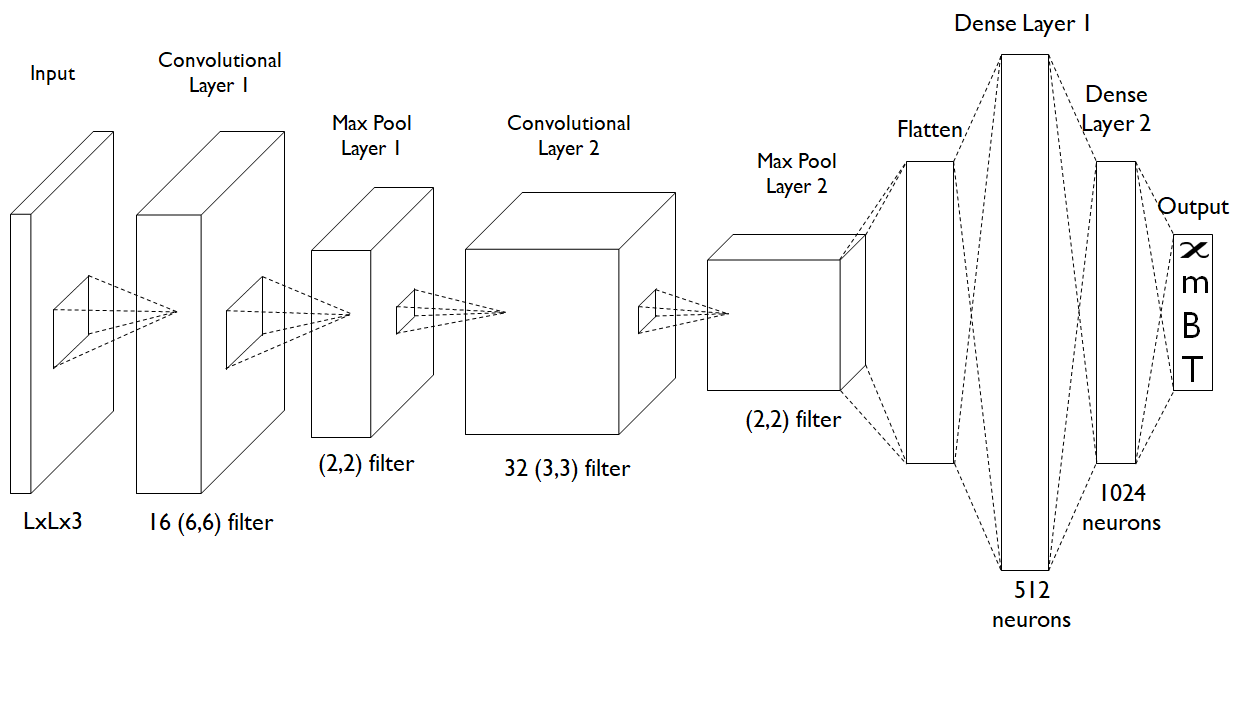
\includegraphics[scale=0.35]{fig1.png}
\caption{Schematic diagram of the ML architecture we used. See main text for explanation.}\label{fig:1}
\end{figure}

\begin{figure}[h]
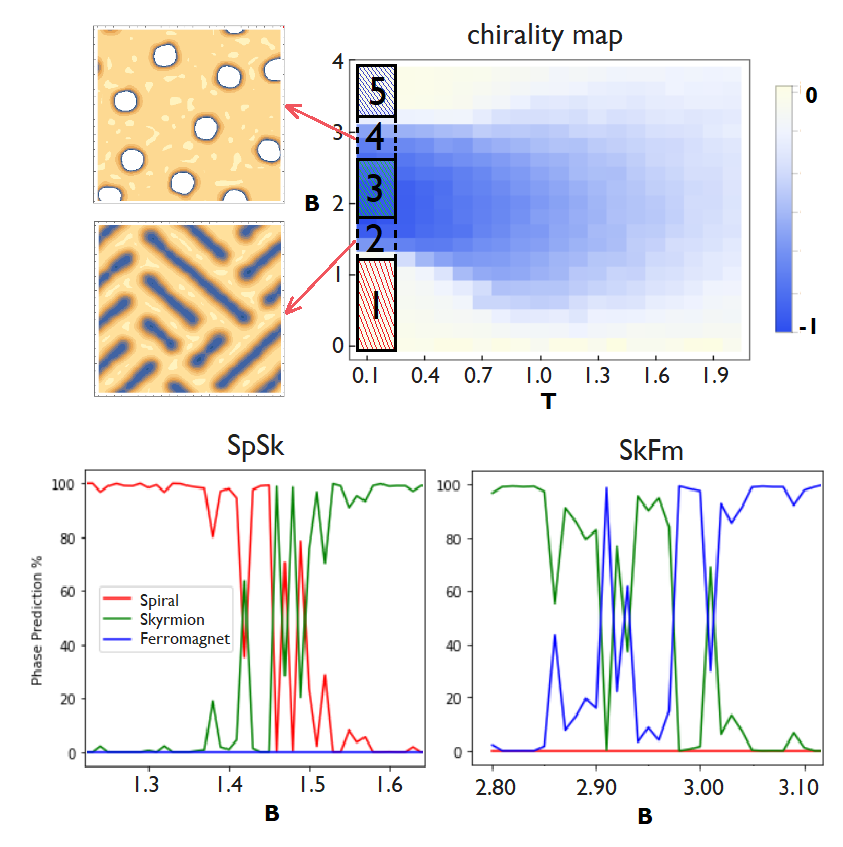
\includegraphics[scale=0.5]{fig2.png}
\caption{(top) Spin chirality [$\chi$ in Eq. (\ref{eq:m-and-chi})] in the $(T,B)$ plane obtained by MC calculation on the HDMZ Hamiltonian (\ref{eq:HDMZ}). Color scale represents the normalized value of the chirality. Boxes 1, 3, and 5 (2 and 4) represent regions where training (testing) data were taken for label predictions. Two configurations on the left show a typical SpSk and SkFm mixed state, respectively. The $z$-component of the local magnetization is used for the plots. (bottom) Probability of phase predictions in the SpSk and SkFm phases. The numbers represent averages over the testing set in the temperature interval $T\in[0.03,0.25]$ at the same $B$ value. The irregularities are not artifacts of the small data size.}\label{fig:2}
\end{figure}

Although we do not focus on the phase identification problem in this work as other reports already exist in the literature~\cite{russian18}, we do note an interesting aspect of the model (\ref{eq:HDMZ}) which is absent in most models studied in recent years and not adequately addressed in the previous work~\cite{russian18}. It is the substantial co-existence region both for the mixture of spiral and skyrmion (SpSk), and of skyrmion and ferromagnetic (SkFm) phases. These five states (Sp, SpSk, Sk, SkFm, Fm) are indicated as boxes numbered 1 through 5 in Fig. \ref{fig:1}. To see how the ML would fare against such a conspicuous mixed phase, we first did the ML training for MC configurations drawn from boxed regions 1, 3, 5 (three pure states). One-hot encoded labels were used to represent different phases: (1,0,0) for Sp, (0,1,0) for Sk, and (0,0,1) for Fm. Afterwards, configurations drawn from boxes 2, 4 (two mixed states) were fed to the program, demanding that it decides which of the three phases the input image belonged. Binary cross entropy was used as the loss function. The answers given for each test configuration by the machine were averaged over and shown as probabilities for Sp, Sk, and Fm phases  in Fig. \ref{fig:2}(b) and (c). Despite the fact that each data point in the figure represents an average over $2,000$ test configurations and that extremely fine steps in magnetic field $\Delta B= 0.01$ was used, the final results are far from being smooth. Removing the CNN filters did not smooth the outcome either. In contrast, a smooth variation in the probability from 1 (ordered phase) to 0 (disordered phase) was found in models with a second-order phase transition \cite{wang16,melko17,tanaka17,scalettar17,wetzel17,kim18,zhai17,scalettar17,beach18}.
Apparently, the very different ways in which the standard DNN algorithm perceives the mixed phases near the first-order phase transition from the critical states around the second-order transition was not noted in earlier investigation of the same model~\cite{russian18}. 

After all, the main characteristics of the phase diagram in the model (\ref{eq:HDMZ}) are the average spin chirality and the magnetization, defined respectively as
%
\ba
\chi = {1\over N} \sum_i  ( \v n_i \cdot \v n_{i+\hat{x}} \times \v n_{i+\hat{y}} ) ,  ~~
m = {1\over N} \sum_i n_i^z .  \label{eq:m-and-chi} \ea
%
We propose that, instead of training the algorithm on the basis of {\it labels} of configurations such as Sp, Sk, or Fm, we do so on their {\it features} such as $\chi$ and $m$. An ML algorithm capable of predicting $(\chi, m)$ correctly for an input experimental image, for example, would be of greater pragmatic value since it can give quantitative characterization of the physical system under study.

\begin{figure}[h]
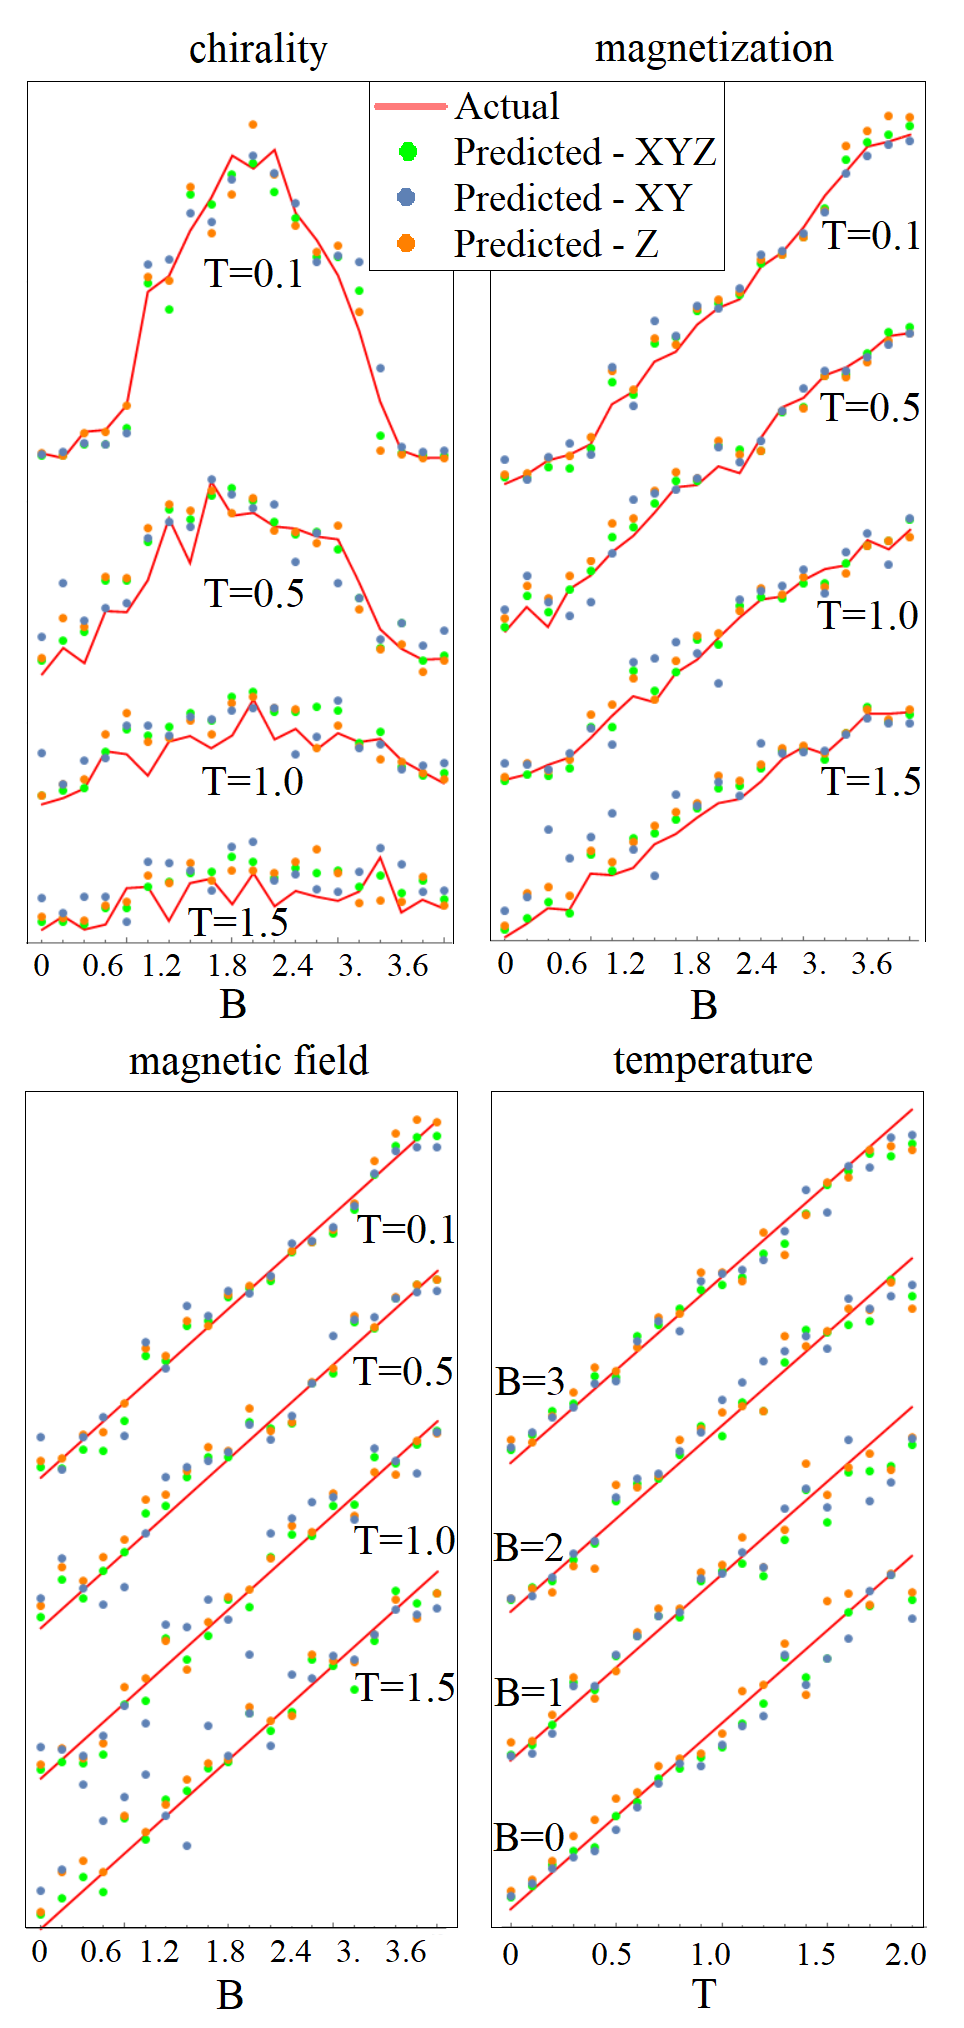
\includegraphics[scale=0.35]{fig3.png}
\caption{Machine-predicted values of $(\chi, m, B, T)$ compared to their actual values in red. Predicted values are obtained from algorithms trained on the full $x,y,z$, $xy$-only, and $z$-only components of the local magnetization. Different curves are offset for clarity.}\label{fig:3}
\end{figure}

Differently from the previous label-learning scheme,  mean-squared error function was used as the loss function. Training configurations were drawn from the entire phase diagram in Fig. \ref{fig:1}. After training, a fresh set of 40,000 configurations were generated to compare the machine-predicted $(\chi,m)$ against the actual values calculated independently with Eq. (\ref{eq:m-and-chi}). We pick one test configuration at a time and compute its $(\chi, m)$ from the formula (\ref{eq:m-and-chi}), and compare it to the machine-predicted values. Shown in the first row of Fig. \ref{fig:3} are the calculated and machine-predicted values of $(\chi, m)$. Three different types of data sets were used for training and testing, with equally good predicted values. Bottom row of Fig. \ref{fig:3} shows predicted $(B,T)$ values from three different training schemes, all with similar accuracy.

Successful as these exercises are, $(\chi, m)$ are both mechanical quantities that might have been calculated with ease by the formula (\ref{eq:m-and-chi}). We therefore ask if external parameters like the temperature ($T$) and the magnetic field ($B$) at which the images were generated can be correctly predicted as well. These are quantities that cannot be read off directly from the input data of spin orientations. Nevertheless, Fig. \ref{fig:2} shows $(T,B)$ values predicted by the algorithm after training to be very close to the actual values. Again, no averaging is done for the plot. Each plot point comes from a single test configuration. It is gratifying that ML works well to predict physical quantities of quite different nature: mechanical and thermodynamic. The trained algorithm has successfully figured out a recipe to extract $(\chi, m, B, T)$ values associated with each image of spin configuration.

Ultimately it will be useful to apply the procedure to the input image obtained in {\it actual experiments}. Let's say we extract local magnetization $\v n_i$ through some imaging technique. Feeding them as inputs to the ML algorithm will correctly predict various features $(\chi, m, B, T)$. Once again, however, there will be little point in doing ML analysis if all of the local magnetization, as well as the external parameters $(T,B)$, were accessible experimentally.  The ML can be of substantial use, however, if some of these information is unavailable or lost.

Consider two prominent imaging techniques currently under use to study skyrmion matter: Lorentz transmission electron microscopy (LTEM) \cite{tokura10} and magnetic force microscopy (MFM) \cite{pana17}. Each of them specializes in imaging the in-plane $(n^x_i , n^y_i )$ and perpendicular ($n^z_i$) components of the local magnetization. The data provided by LTEM and MFM is thus $xy$- and $z$-type, respectively.  Given the raw data, it is impossible to determine the spin chirality directly as it requires the knowledge of all three components of $\v n_i$, or $xyz$-type data set. With the LTEM data it is impossible to read off the average magnetization either. We claim that the situation can be remedied by coupling the experimental data with the properly trained ML program.

Previously we mentioned the excellent prediction for $(\chi, m, B, T)$ made by the ML program trained on the full $xyz$-type data. This time, we perform a new set of training procedures by feeding only the $xy$- or $z$-component of the configuration. The same set of $(\chi, m, B, T)$ data is used for all three types of training: $z$, $xy$, and $xyz$. With three different kinds of ML programs at hand, we feed testing configurations consisting of $z$, $xy$, and $xyz$ components of the magnetization, respectively, and demand that each program make predictions for $(\chi, m, B, T)$. As shown in Fig. \ref{fig:2}, there is virtually no difference in the accuracy of the predicted values of $(\chi, m, B, T)$ for all three types of training and testing data sets. Replace the training data with the experimentally obtained images of either $z$-type (MFM) or $xy$-type (LTEM), one would be making ML predictions on the basis of actual experimental data.

Experimental situation is still more complicated than what the simplified model (\ref{eq:HDMZ}) captures. A most obvious complication is the disorder effect, coming from inhomogeneities in the interaction parameters of the Hamiltonian or local anisotropy terms we ignored so far. The predictive capacity of ML would be much reduced if the it works well only on test  configurations generated by the exact same model from which training set was generated in the first place. Luckily, the numerical experiment presented below shows that the ML program trained on the pristine model continues to give reliable predictions for test configurations obtained from models with disorder. Replace the dirty model configurations by the actual experimental images (which always come from imperfect samples), we come to conclude that ML could give reliable predictions from messy experimental data as well.

\begin{figure}[t]
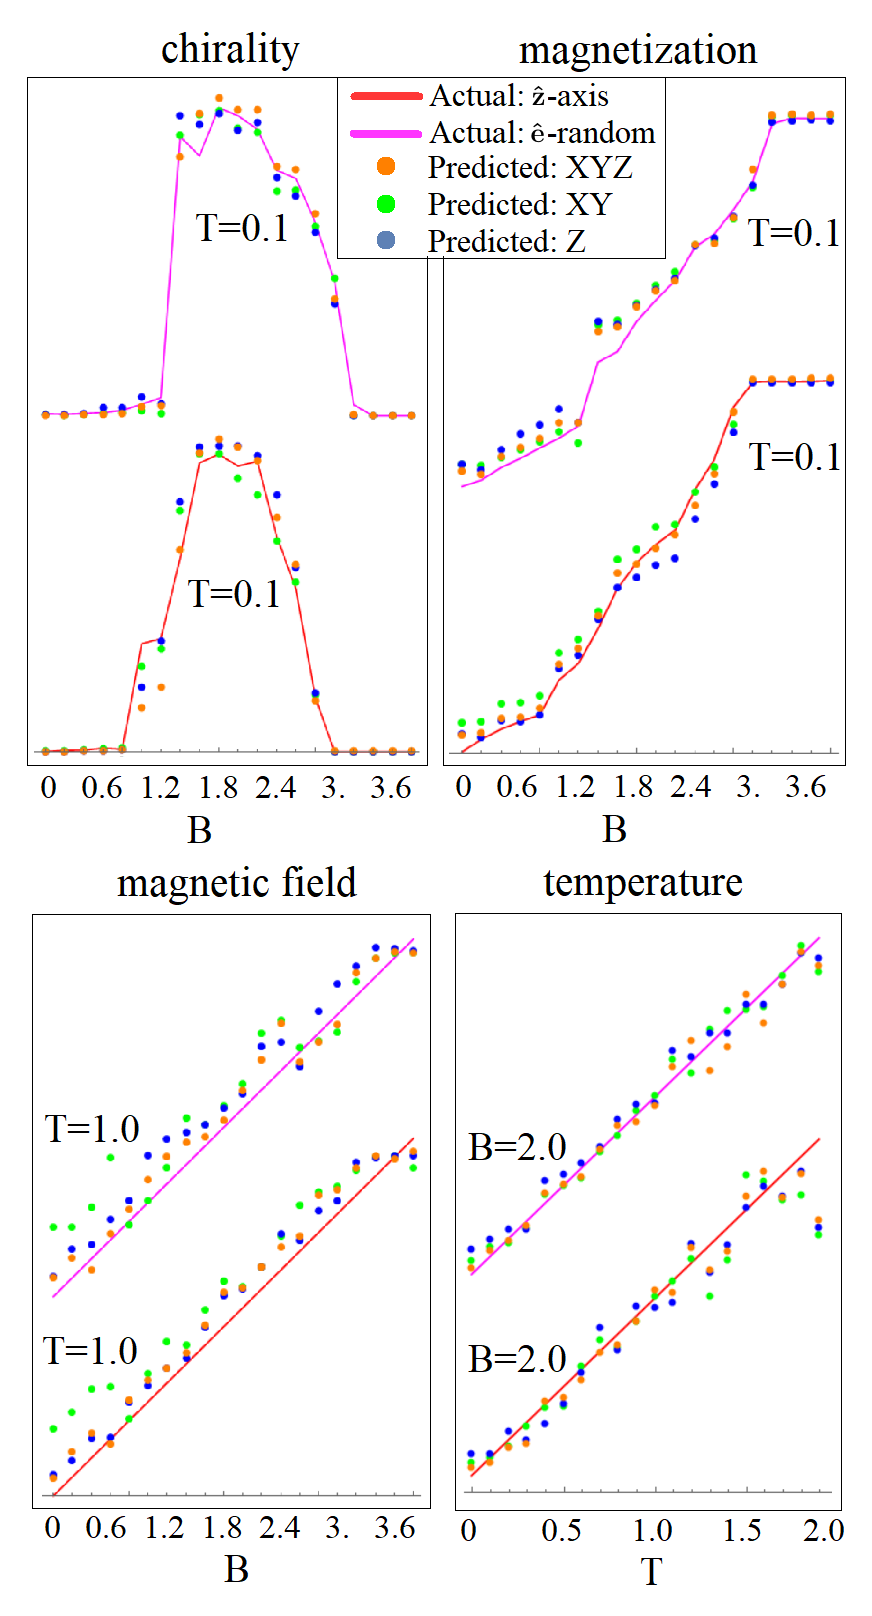
\includegraphics[scale=0.36]{fig4.png}
\caption{ML prediction of $(\chi, m, B, T)$ for MC configurations generated by $H_{\rm HDMZ}+ H_1$, and $H_{\rm HDMZ} + H_2$, with $(K,p)=(1, 0.5)$ for both models.  All three input data types ($z$, $xy$, $xyz$) give equally good predictions.} \label{fig:4}
\end{figure}


We consider two kinds of disorder terms to add to the HDMZ Hamiltonian (\ref{eq:HDMZ}):
%
\ba H_{1} = -K \sum_{i \in {\rm ran}} (\hat{z} \cdot \v n_i )^2 , ~~ H_2 = - K \sum_{i \in {\rm ran}} (\hat{e}_i \cdot \v n_i )^2 .  \ea
%
In $H_1$, easy $z$-axis magnetic anisotropy of strength $K$ is added at the random sites occupying a fraction $p$ of the whole lattice. In $H_2$, the anisotropy orientation $\hat{e}_i$ is also random. A new batch of test configurations has been generated by doing MC on either  $H_{\rm HDMZ} + H_1$ or $H_{\rm HDMZ} + H_2$. We do not, however, generate a new ML algorithm trained on these new configurations. The newly-generated MC configurations are simply fed to the existing program, trained on the disorder-free model, and predictions for $(\chi, m, B, T)$ are demanded. As before, three different input types ($z$, $xy$, and $xyz$) have been used on three different ML programs. Figure \ref{fig:4} shows the outcome of such investigation. In essence, actual $(\chi, m, B, T)$ values of the test configurations with disorder are faithfully reproduced across all three data and ML types. Our numerical experiment suggests that the predictive power of ML remains universal across a range of disorder potentials.

Having presented a diversity of ML-related analysis of the HDMZ model and impurity generalizations, we conclude with a specific recipe how to integrate ML as an effective tool for analysis of the experimental data. Firstly, any experimental image of spirals or skyrmions obtained by LTEM or MFM can be coarse-grained and re-sized so that the relevant length scale becomes the same as the one used in the training program. If necessary, one can try several different coarse-graining length scales for treating the raw experimental data until the most efficient prediction by ML is achieved. After this preparation stage, one can reconstruct missing information such as the spin chirality and magnetization, not provided by the raw experimental data, with the help of ML. The magnetization thus extracted can be compared to the value obtained in the direct magnetization measurement. Spin chirality, on the other hand, does not have an obvious coupling to an experimental probe. Although it is said that topological Hall effect originates from the skyrmions, the relation between the number of skyrmions or the spin chirality and the Hall effect is not rigorous. The ML prediction of spin chirality can be a valuable source of information not directly attainable in any experiments. Our impurity calculation also supports that ML program trained on one paradigmatic model Hamiltonian such as (\ref{eq:HDMZ}) will give robust predictions for physical systems corrupted by various impurity effects. 

This work was supported by Samsung Science and Technology Foundation under Project Number SSTF-BA1701-07.

\begin{thebibliography}{99}

\bibitem{melko16} G. Torlai and R. G. Melko, Phys. Rev. B {\bf 94}, 165134 (2016).

\bibitem{wang16} L. Wang, Phys. Rev. B {\bf 94}, 195105 (2016).

\bibitem{melko17} J. Carrasquilla and R. G. Melko, Nat. Phys. {\bf 13}, 431 (2017).

\bibitem{melko17b} P. Ponte and R. G. Melko, Phys. Rev. B {\bf 96}, 205146 (2017).

\bibitem{melko17c} A. Morningstar and R. G. Melko, arXiv:1708.04622 (2017).

\bibitem{tanaka17} A. Tanaka and A. Tomiya, J. Phys. Soc. Jpn. {\bf 86}, 063001 (2017).

\bibitem{scalettar17} W. Hu, R. R. P. Singh, and R. T. Scalettar, Phys. Rev. E {\bf 95}, 062122 (2017).

\bibitem{wetzel17} S. J. Wetzel and M. Scherzer, Phys. Rev. B {\bf 96}, 184410 (2017).

\bibitem{wetzel17b} S. J. Wetzel, Phys. Rev. E {\bf 96}, 022140 (2017).

\bibitem{iso18} S. Iso, S. Shiba, and S. Yokoo, Phys. Rev. E {\bf 97}, 053304 (2018).

\bibitem{kim18} D. Kim and D.-H. Kim, Phys. Rev. E {\bf 98}, 022138 (2018).

\bibitem{zhai17} C. Wang and H. Zhai, Phys. Rev. B {\bf 96}, 144432 (2017).

\bibitem{beach18} M. J. S. Beach, A. Golubeva, and R. G. Melko, Phys. Rev. B {\bf 97}, 045207 (2018).

\bibitem{zhai18} C. Wang and H. Zhai, arXiv:1803.01205 (2018).

\bibitem{russian18} I. A. Iakovlev, O. M. Sotnikov, and V. V. Mazurenko, arXiv:1803.06682v1 (2018).


\bibitem{nagaosa-review} N. Nagaosa and Y. Tokura, Nature Nanotech. {\bf 8}, 899 (2013).

\bibitem{skyrmion-book} J. P. Liu, Z. Zhang, and G. Zhao, {\it Skyrmions: topological structures, properties, and applications} (CRC Press, 2016)

\bibitem{jiang-review} W. Jiang, G. Chen, K. Liu, J. Zang, S. G. E. Velthuis, and A. Hoffmann, {\it Phys. Rep.} {\bf 704},1 (2017).

\bibitem{fert-review} A. Fert, N. Reyren, and V. Cros, Nature Reviews Materials {\bf 2}, 17031 (2017).

\bibitem{han-book} J. H. Han, {\it Skyrmions in Condensed Matter}  (Springer, 2017).

\bibitem{bishop} C. M. Bishop, {\it Pattern Recognition and Machine Learning} (Springer, 2006).
 
\bibitem{goodfellow} I. Goodfellow, Y. Bengio, and A. Courville, {\it Deep Learning} (The MIT Press, 2016).

\bibitem{ng} For example, Andrew Ng's online deep learning lecture can be found at https://www.coursera.org/specializations/deep-learning 

\bibitem{tokura10} X. Z. Yu, Y. Onose, N. Kanazawa, J. H. Park, J. H. Han, Y. Matsui, N. Nagaosa, and Y. Tokura, Nature (London) {\bf 465}, 901 (2010).

\bibitem{pana17} A. Soumyanarayanan, {\it et al}., {\it Nat. Mat.} {\bf 16}, 898 (2017).

%\bibitem{SM} Supplementary Material
%\bibitem{zhai18b} Y. Wu, P. Zhang, H. Shen, and H. Zhai, Phys. Rev. A {\bf 98}, 010701 (2018).

\end{thebibliography}

%\bibliographystyle{apsrev}
%\bibliography{reference}

\end{document}

The model $H(K,p) = H_{\rm HDMZ} + H_K$ represents an adiabatically connected family of Hamiltonians as long as $K$ is sufficiently small compared to other energy scales. It is interesting to ask whether the ML algorithm, trained solely on  configurations drawn from $H(0,0)= H_{\rm HDMZ}$, can have predictive power over those generated from arbitrary $H(K,p)$. It is also a pragmatic question, when it comes to addressing the machine's predictive power over the experimental data, as real materials are never free of inhomogeneities and one does not have the {\it a priori} knowledge of the governing Hamiltonian. A large number of configurations at the $(K,p)$ values shown in Table \ref{tab:PBC} was generated by MC and tested by the ML algorithm, previously  trained solely on the pristine Hamiltonian $H_{\rm HDMZ}$. As shown as extensive data sets in SM, very good fits of all features $(\chi, m, B, T)$ were obtained. The error in the prediction can be quantified by measuring $\Delta X \! \equiv \!  \sum_{i=T,B} \! | X_{\rm pred.} \! - \! X_{\rm act.} | / 400 $, where 400 refers to the total number of $(T,B)$ steps used in the generation of the test set, and $X=\chi, m, B, T$. Table \ref{tab:PBC} shows the mean errors in $(\chi, m, B, T)$ for several $(K,p)$ values. Both $\Delta \chi$ and $\Delta m$ remain less than 0.05 as $K$ grows from 0 to 2 (recall $J=1$ and $D=\sqrt{6}$). Note that $\chi$ and $m$ have the maximum size of 1. On the other hand, there is a systematic growth in $\Delta B$ and $\Delta T$ as $K$ becomes larger.

\begin{table}[htb]
\begin{tabular}{ | ccc || ccc  cc  cc  cc |}
\hline
 & $(K, p)$ & & & $\Delta\chi$ &  & $\Delta m$ &  & $\Delta B$ & & $\Delta T$ & \\ \hline
 & $(0,0)$  &  & & 0.026 & & 0.027 & & 0.032 & &  0.028 & \\ \hline
 & $(1,0.5)$ & & & 0.030 & & 0.029 & & 0.060 & & 0.037 & \\ \hline
 & $(1,1)$   & & & 0.038 & & 0.024 & & 0.087 & & 0.066 & \\ \hline
 & $(2, 0.5)$ & & & 0.042 & & 0.025 & & 0.083 & & 0.064 & \\ \hline
 & $(2,1)$ & & & 0.042 & & 0.024 & & 0.152 & & 0.100 & \\ \hline
\end{tabular}\label{tab:PBC}
\caption{Averaged variance between predicted and actual values of $(\chi, m, B, T)$.}
\end{table}


We plot predicted values $B_{\rm pred.}$ against the actual $B$ in Fig. \ref{fig:4}(a) for several $(K,p)$'s. There is an approximate linear relationship in $B_{\rm pred.}$ against $B$, at least until $B_{\rm pred.}$ reaches saturation, with the slope that grows almost linearly with $K$, as shown in Fig. \ref{fig:4}(b). The effect of the added anisotropy can be qualitatively understood within the mean-field picture by replacing $K  \sum_{i \in {\rm random}}  (n^z_i )^2$ with $2K p m \sum_{i \in L^2} n^z_i$, where $p$ is the impurity fraction. Assuming the magnetization $m$ depending linearly on $B$, $m = \alpha B$, the overall effect of the random anisotropy term is to replace the external field $B$ by the effective one, $B_{\rm eff} = (1+ 2K p\alpha ) B$. The machine, having been trained solely on pristine $H_{\rm HDMZ}$, knows nothing of the impurity effect {\it a priori} and ``erroneously" predicts the renormalized $B_{\rm eff}$ for the input, thereby incidentally divulging the discrepancy between the training and testing Hamiltonian.

Such expectations are consistent with our numerical analysis of Fig. \ref{fig:4}(b), showing almost linear increase in the slope of $B_{\rm pred.}$ with $K$. To further prove this picture we obtain $\alpha$ independently from linear fits to predicted $m$ values such as shown in SM Fig. 4. The two ways of extracting the susceptibility $\alpha$ agree very well. The $\sim 2$ times difference in the estimated slopes for $p=0.5$ and $p=1$ data are consistent with the mean-field picture of $B_{\rm eff}$, as shown in Fig. \ref{fig:4}(b). The under-estimation of the temperature by the machine, as shown in SM figure 2, can be also understood, qualitatively, as a result of $K$ having the tendency to stiffen the spins and align them. At the same bare temperature $T$, configurations generated at finite $K$ tend to have more alignment of spins, which is ``erroneously" seen by the machine to be the consequence of lesser effective temperature $T_{\rm eff} < T$. Our numerical experiment demonstrates how well the neural network can respond to perturbations in the model~\cite{zhai18b}.


